\subsection{Gaia}
Criou-se um \emph{middleware} (Gaia OS) com o objetivo de dar suporte ao desenvolvimento e execução de aplicações em \emph{Active Spaces}, ambientes com sistemas interativos. Foi projetado para ter uma infraestrutura distribuída que coordena entidades de software e dispositivos heterogêneos em um \emph{smart space}. O Gaia OS expõe serviços para buscar e utilizar recursos presentes no ambiente, ter conhecimento do contexto e provê um \emph{framework} para desenvolver aplicações móveis sensíveis ao contexto, que conheçam os recursos disponíveis, utilizem múltiplos dispositivos e possuam como foco o usuário~\cite{gaia2002}.

\emph{Active Spaces} são espaços físicos como escritórios, salas de conferência, casas, hospitais, campi universitários, cidades, etc, que possuam dispositivos integrados ao ambiente. Tais dispositivos devem prover e obter informações sobre usuários presentes no ambiente, auxiliando-os e/ou facilitando a realizar tarefas que eles não poderiam sem os dispositivos.

\begin{figure}[ht]
\center
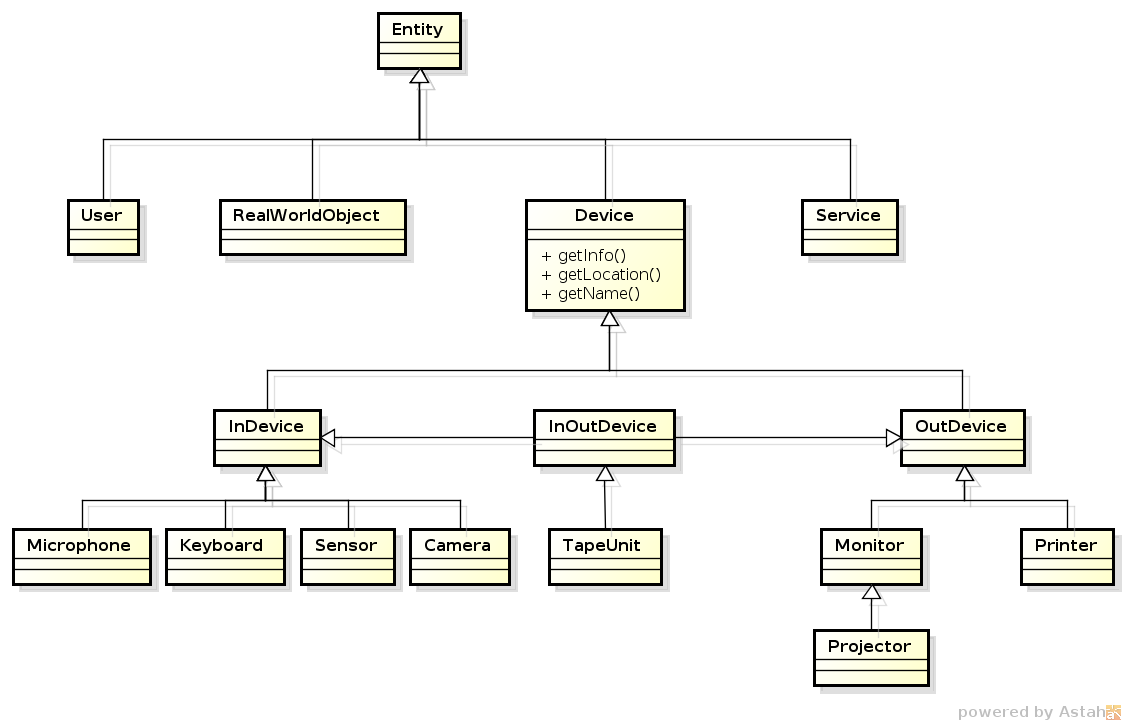
\includegraphics[scale=0.5]{imagens/gaia-devices}
\caption{Diagrama de Classes Simplificado~\cite{gaiaDevices}}
\label{fig:gaiaClassDiagram}
\end{figure}

Desenvolveu-se também um \emph{framework} para a interação entre dispositivos heterogêneos que permite a representação das interfaces dos dispositivos com diferentes níveis de detalhe e especialização. Tais interfaces são definidas utilizando IDL(\emph{Interface Description Language}), que permite a construção de \emph{drivers} de dispositivos em qualquer linguagem de programação garantindo uma facilidade de integração com diferentes dispositivos.

A figura~\ref{fig:gaiaClassDiagram} mostra o diagrama de classes simplificado do projeto. Pode-se observar que a classe \emph{Device} foi especializada em outras classes: \emph{InDevice} e \emph{OutDevice}. Os dispositivos de entrada foram ainda especializados em: \emph{Microphone}, \emph{Keyboard}, \emph{Sensor} e \emph{Camera}, enquanto os dispositivos de saída foram especializados em: \emph{Monitor}, \emph{Printer} e \emph{Projetor}. A interface para dispositivos de entrada e saída foi especializada na classe \emph{Fita}.